%************************************************
\chapter{Data Analysis at the LHC}\label{ch:introduction}
%************************************************
The LHC produces -at design parameters- over 600 millions collisions ($\approx 10^9$ collisions) proton-proton per second in ATLAS or CMS detectors. The amount of data collected for each event is around 1 MB (1 Megabyte). This means that we are reaching 1 PB/s (1 \emph{Peta}byte/second) of data--far too much for any detector data acquisition system to handle.

The trigger systems alleviate the problem by reducing the amount of data by a factor of 1000 or 10000; despite this, the constant need of cutting-edge resources and solutions, both in hardware and software, have been driving extremely fruitful research in the history of the LHC.

One major necessity, whose importance and scale may not be appreciated by people outside of the field, is the one for \emph{simulations}.

\section{The necessity of simulations}

First of all, why do we need simulations in the first place?
The simulation is a crucial aspect of any high energy physics experiments. In CMS it is used both
at analysis level and for testing the algorithms before deployment with data. The simulation targets relatively rare processes originating from a hard interaction between two
proton components, which are signal or background for specific analyses. Single particles
or hadronic jets can also be simulated for specific purposes.

Simulations are a necessity if we have to test a physical theory: we need to know what reality would look like if the proposed theory was true or not. Then we can check which hypothesis our data looks like, and we can either validate or disprove the theory.

Without a proper simulation, we also would not know the expected performance of the detector and the regions of interest for our process, making it impossible to correctly operate the apparatus and obtain reasonable results.

\section{Modelling an event}

There are three major, distinct steps in modelling a physical event at CMS. The first one is more generally related to the physical theories and calculations, while the other two are specific to the CMS detector.

\subsection{Event generation}

The first step to any good simulation is called \emph{generation}, that is all the calculations based on Quantum Chromodynamics which describes how the quarks and gluons inside the protons scatter off one another, how they might create new particles, and how those new particles behave after they have been created. 

Proton-proton collisions are very complex and difficult to model accurately. Protons are
composed of 3 quarks, called \emph{valence} quarks, by virtual gluons and virtual quark anti-quark
pairs coming from gluon splitting. All constituents of hadrons are generically called \emph{partons}.
During high energy collisions, the protons behave as a collection of free partons and the
hard scattering can be described at the level of parton interactions. The hadronic cross
section $\sigma_{pp}$ is calculated based on the QCD \emph{factorization} theorem. The factorization theorem
states that the hadronic cross-section $\sigma_{pp}$ is a convolution of the partonic cross section  $\hat{\sigma}_{ij}$ with the parton distribution functions (PDFs) $f_i(x)$:

\[
\sigma_{pp} = \int_{x_{min}}^1 dx_1 dx_2 \sum_{i,j}f_i(x_1)f_j(x_2)\hat{\sigma}_{ij}(x_1 p_1, x_2 p_2)
\]

where function $f_i(x)$ is probability density that a parton of type i has a fraction x of the
hadron energy. The final cross section may be evaluated by the single, non-trivial contributions $\hat{\sigma}_{ij}$.

Apart from the hard interaction, the other constituents of the proton can also interact. This
usually results in a spray of softer particles, called \emph{underlying event} (UE). Any high momentum particle involved in the collision will emit additional hard QCD radiation. Radiation
from particles before the hard interaction is called \emph{initial-state-radiation} (ISR), whereas radiation off particles produced in the collision is called \emph{final-state-radiation} (FSR). Quarks and gluons can emit additional radiation via the strong interaction. All the quarks
and gluons go through the hadronization process, forming colorless hadrons. Finally, unstable particles are going to decay. A representation of all these elements is shown in Figure \ref{fig:evgen}.          

\begin{figure}
    \centering
     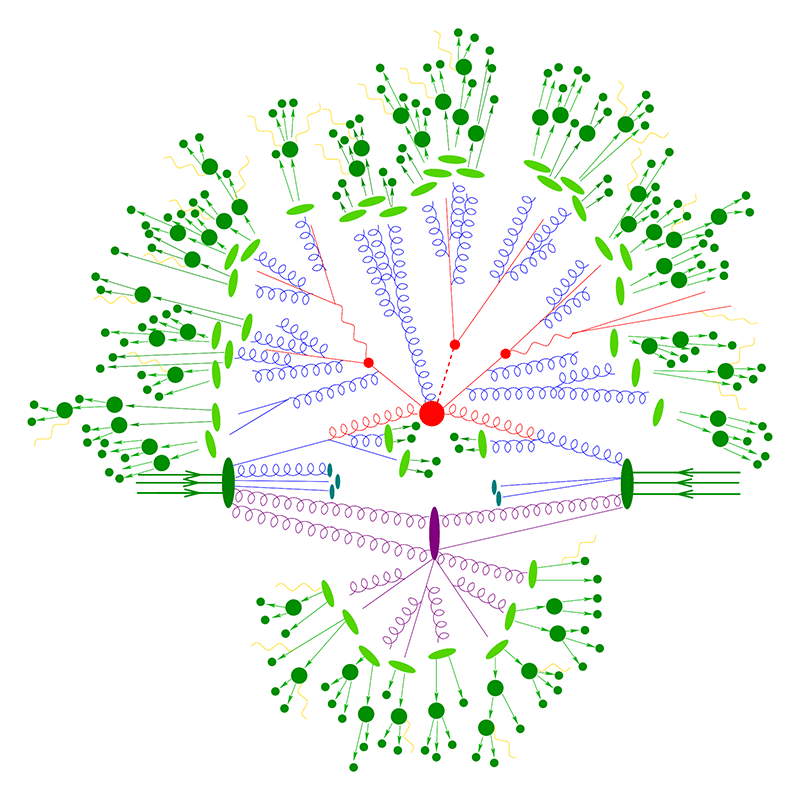
\includegraphics[width=.65\linewidth]{gfx/ch2/event_800px.png}
    \caption[Event generation]{ Representation of a proton-proton collision event. The red part includes the hard interaction and the decay of the products. Initial and final state radiation are in blue. A secondary
interaction can take place, in purple, before the final-state partons hadronize. The hadronization is
represented by the green blobs, and the hadron decay in dark green. Photon radiation is in yellow. From \cite{evgen}.}
    \label{fig:evgen}
\end{figure}


All the various parts involved in this step can be summarized as:

\begin{outline}
    \1  The PDFs that are phenomenological functions computed using experimental information;
    \1  the hard scattering, computed perturbatively order by order;
    \1  the parton \emph{showering}, used to simulate additional emissions in perturbative QCD;
    \1   the hadronization, describing the transition from colored particles to hadrons, treated
        using phenomenological models;
    \1   the decay of unstable particles, modeled based on experimental data.
    
\end{outline}

The first two are usually included in \emph{Matrix Elements generators}, while the last three are
included in Parton Showering programs. Both use Monte Carlo techniques; some popular multi-purpose generators include \texttt{Pythia8}, \texttt{MadGraph} and \texttt{Sherpa}.

We can thus obtain a complete description of all the (stable) particles that come out of a collision between two protons under our theory only after a complex process involving several months of modelling and calculations.

\subsection{Detector Simulation through GEANT4}

Now that we have the particles resulting from our process, we must take the detector into account. This means simulating all the interaction processes that are going to happen between particles and matter by moving them through the detector one by one and modelling the detector’s response to each one of the particles as it goes. 
Undoubtedly, the de-facto standard for such a task is the \texttt{Geant4} toolkit (see \cite{AGOSTINELLI2003250}). It is intended to simulate the passage of particles through matter and it includes a complete range of functionality including tracking, geometry, physics models and hits. The physics processes offered cover a comprehensive range, including electromagnetic, hadronic and optical processes, a large set of long-lived particles, materials and elements, over a wide energy range starting, in some cases, from 250 eV and extending in others to the TeV energy range. It has been designed and constructed to expose the physics models utilised, to handle complex geometries, and to enable its easy adaptation for optimal use in different sets of applications. The toolkit is the result of a worldwide collaboration of physicists and software engineers, created exploiting software engineering and object-oriented technology and implemented in the \texttt{C++} programming language.

\begin{figure}
    \centering
     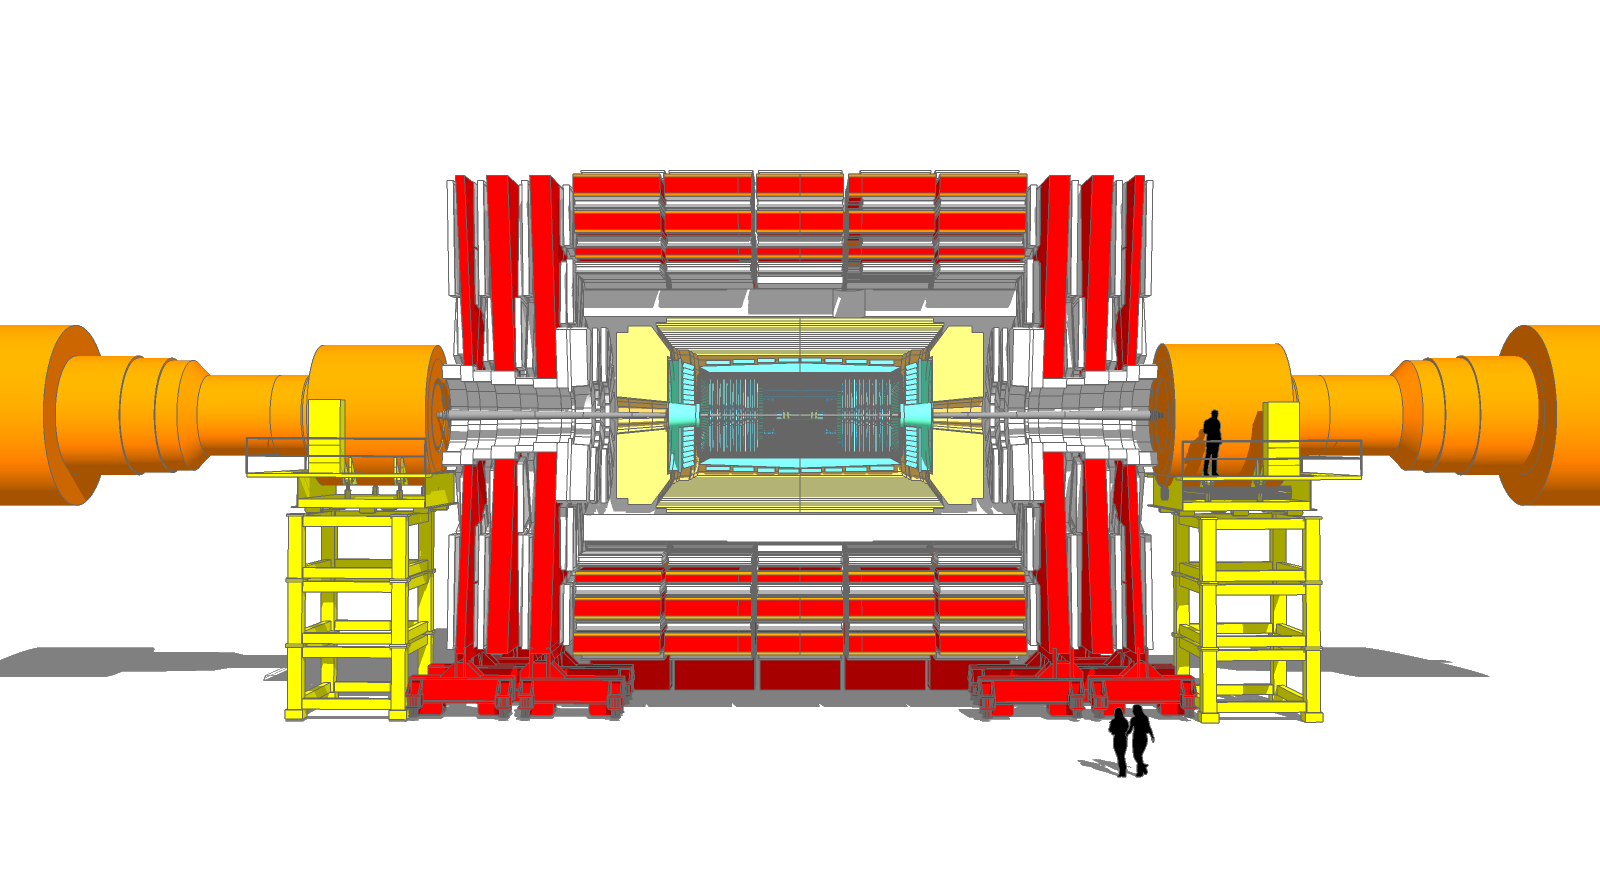
\includegraphics[width=\columnwidth]{gfx/ch2/cms_160518_01_Scene_2.png}
    \caption[CMS model]{ Representation of the CMS detector based on the actual \texttt{Geant4} CMS Detector Description. It accurately and precisely reproduces the geometry of all CMS detector subsystems, including the geometries of the original CMS detector, phase 1 and phase 2 upgrades.  From \cite{decmod}}
    \label{fig:decmod}
\end{figure}


However, \texttt{Geant4} can only provide us with a description of the single physical processes and materials, so we need to provide him with the actual \emph{detector description} (see Figure \ref{fig:decmod}). Every piece of the detector has to be put together, with the right material assigned to each. We have a detector description with over five million (!) volumes and about 400 different materials (from Xenon to Argon to Air to Aerogel and Kapton Cable). There are a few heroes of ATLAS who spend a lot of time taking technical drawings (and photographs, because the technical drawings aren’t always right!) of the detector and translating them into something Geant4 can use. You can’t put every wire and pipe in – the simulation would take an eternity! – so you have to find shortcuts sometimes. It’s a painstaking process that’s still ongoing today. We continuously refine and improve our description, adding pieces that weren’t important at the beginning several years ago but are starting to be important now (like polyboron neutron shielding in our forward region; few people thought early on that we would be able to model low-energy neutron flux in our detector with Geant4, because it’s really complex nuclear physics, but we’re getting so close to being able to do so that we’ve gone back to re-check that our materials’ neutron capture properties are correct). And sometimes we go back and revise things that were done approximately in the beginning because we think we can do better. This part also involves making a detailed magnetic field map. We can’t measure the field everywhere in the detector (like deep in the middle of the calorimeter), and it takes too much time to constantly simulate the currents flowing through the magnets and their effect on the particles moving through the detector, so we do that simulation once and save the magnetic field that results.
\subsection{Digitization and Reconstruction} 

\subsection{Computing Costs}

\subsection{FastSim}

\section{The NanoAOD format}




%*****************************************
%*****************************************
%*****************************************
%*****************************************
%*****************************************
